\documentclass{beamer}
\usepackage[latin1]{inputenc}
\usepackage{times}
\usepackage{tikz}
\usetheme{Luebeck}
%\usecolortheme{albatross}
\usepackage{amsmath,amsfonts,amsthm,amssymb}
\usepackage{setspace}
\usepackage{Tabbing}
\usepackage{fancyhdr}
\usepackage{lastpage}
\usepackage{extramarks}
\usepackage{chngpage}
\usepackage{soul,color}
\usepackage{graphicx,float,wrapfig}
\usepackage{listings}
\usepackage{float}
\usepackage{subfig}
\usepackage{enumitem}
\usepackage{algpseudocode}
\usepackage{biblatex}
\usefonttheme{professionalfonts}
\setbeamertemplate{navigation symbols}{} 
\definecolor{darkorange}{RGB}{240, 120, 0}

\setbeamercolor{background canvas}{bg=white}
\setbeamercolor{frametitle}{fg=white, bg=darkorange}
\setbeamercolor{normal text}{bg=black,fg=black}
\setbeamercolor{structure}{bg=black, fg=darkorange}

\title{Hashing Slides}
\date{12/5/2018}
\institute{Duke University, ECE / Math}
\author{Chris Tralie}

%\addbibresource{../Bibliography/Alignment_TimeSeries_Curves.bib,../Bibliography/CoverSongs.bib,../Bibliography/Diffusion_Intrinsic_Spectral.bib,../Bibliography/GromovHausdorff_MetricTrees.bib,../Bibliography/MIR_General.bib,../Bibliography/mybib.bib,../Bibliography/Other.bib,../Bibliography/Rhythm.bib,../Bibliography/TDA.bib,../Bibliography/Textbooks.bib,../Bibliography/TimeSeriesGeneral.bib,../Bibliography/VideoProcessing.bib} 

\addbibresource{slides.bib}


\graphicspath{{Figures/}}

\newcommand{\vect}[1]{\boldsymbol{#1}}
\newcommand{\mb}{\mathbf}

\begin{document}

\frame{\titlepage}


\begin{frame}{Theory: Pseudorandom Functions}

\begin{itemize}[label=$\vartriangleright$]
    \item Each key equally likely to map to integer between $0$ and $M-1$
    \item Throw balls blindfolded into bins
\end{itemize}

\begin{figure}
	\centering
	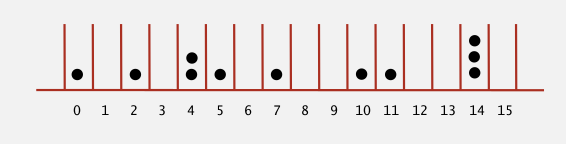
\includegraphics[width=0.8\textwidth]{BinsBalls.png}
\end{figure}

\begin{itemize}[label=$\vartriangleright$]
\uncover<2->{
    \item Birthday paradox: Expect collision after $\approx \sqrt{\pi M/2}$ tosses
}
\uncover<3->{
    \item Expect every bin has $\geq 1$ ball after $\approx M \ln M$ tosses
}
\uncover<4->{
    \item After $M$ tosses, expected most loaded bin has $\Theta(\log M/ \log \log M)$ balls
}
\end{itemize}

\end{frame}




\begin{frame}{C++ Implementation}

\begin{figure}
	\centering
	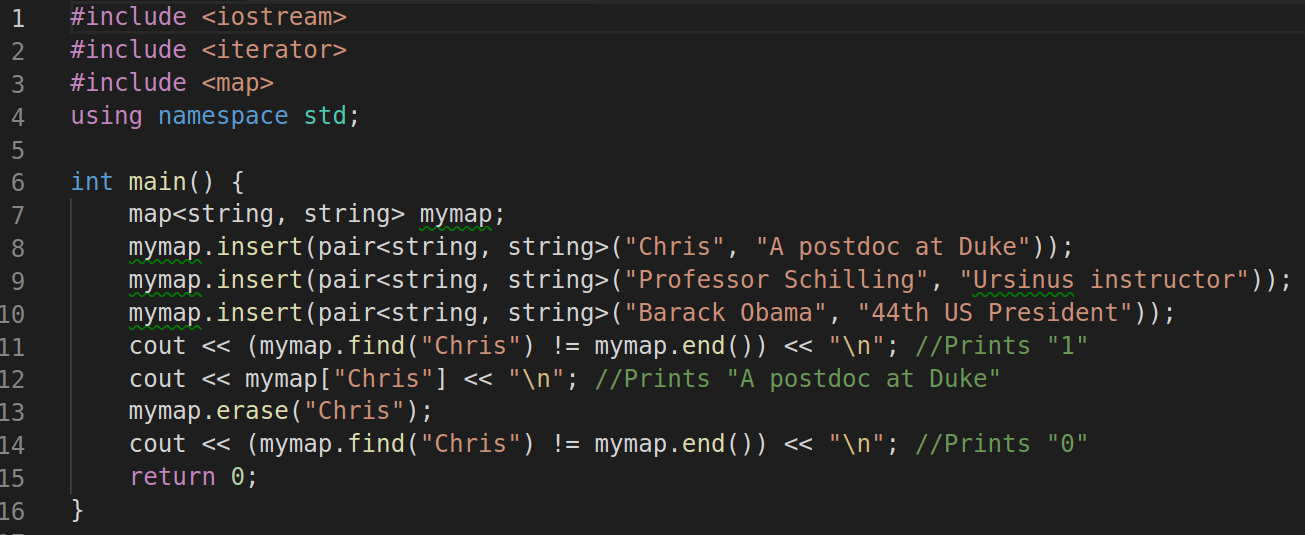
\includegraphics[width=\textwidth]{CPPHash.png}
\end{figure}

\end{frame}



\begin{frame}{Java Implementation}

\begin{figure}
	\centering
	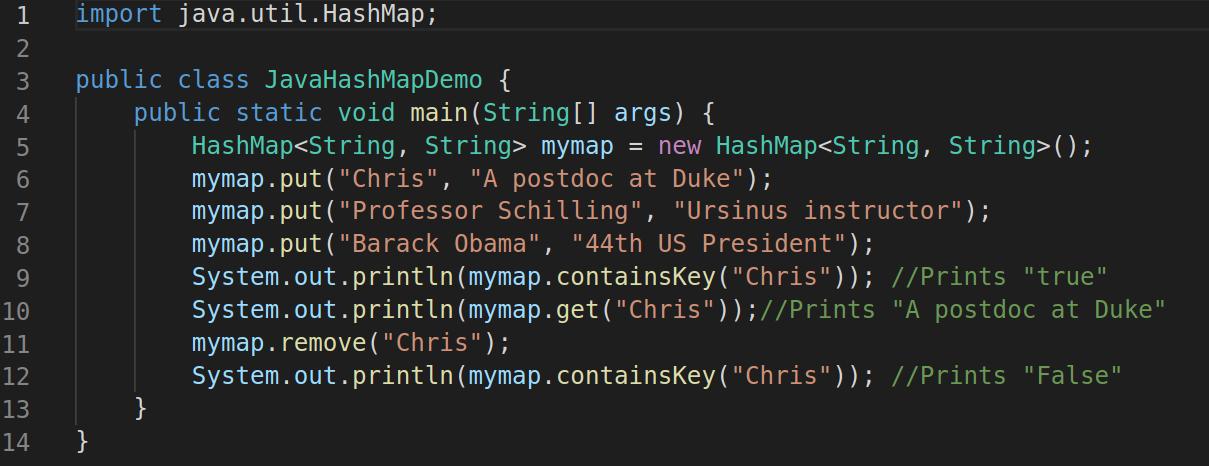
\includegraphics[width=\textwidth]{JavaHash.png}
\end{figure}

\end{frame}


\begin{frame}{Java's scheme}

\begin{figure}
	\centering
	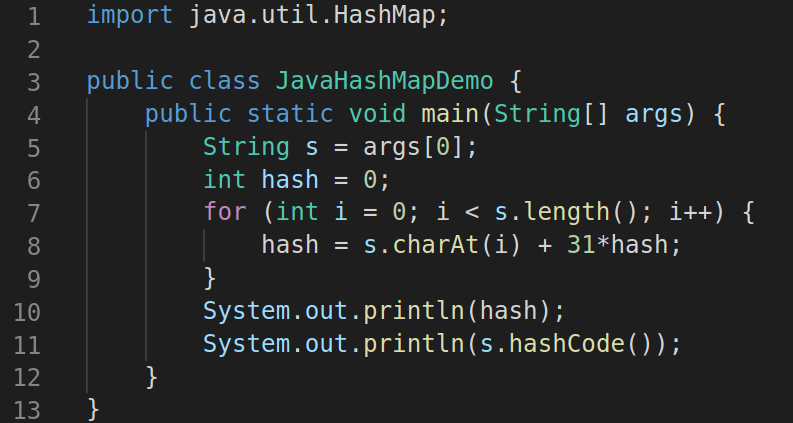
\includegraphics[width=0.8\textwidth]{JavaHash31.png}
\end{figure}

\begin{itemize}
    \item Hello $\rightarrow$ 69609650
    \item Chris $\rightarrow$ 65087095
    \item Ursinus $\rightarrow$ 1501567193
\end{itemize}

\end{frame}


\begin{frame}{Adversarial Attack?}

\uncover<2->{
    \begin{itemize}
        \item More stable: MD4, MD5, SHA-0, SHA-1, SHA-2, WHIRLPOOL, RIPEMD-160
    \end{itemize}
}

\uncover<3->{
    \begin{figure}
	    \centering
	    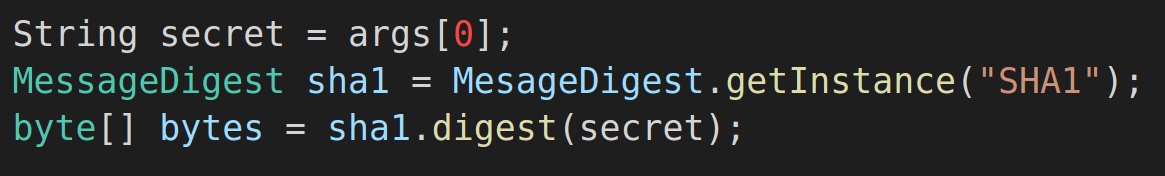
\includegraphics[width=\textwidth]{Sha1.png}
    \end{figure}

}
\end{frame}

\begin{frame}{Applications?}


\end{frame}



\begin{frame}{The Shazam Technique}

\begin{figure}
	\centering
	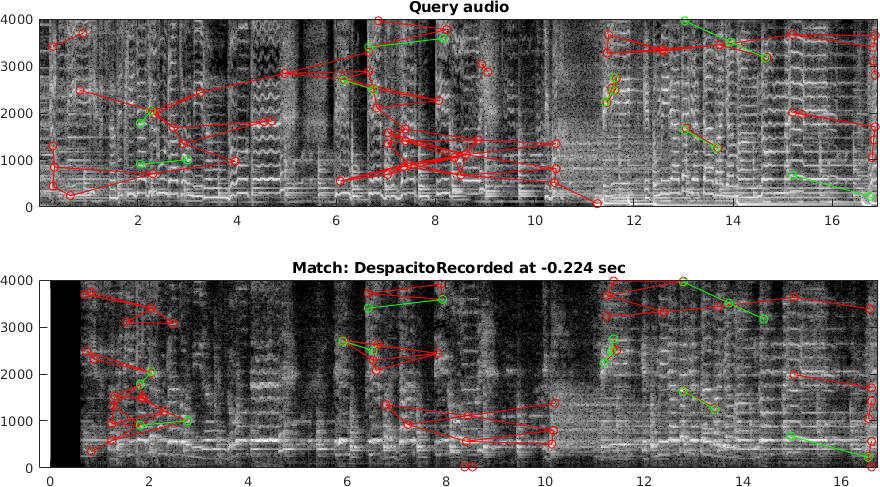
\includegraphics[width=\textwidth]{DespacitoRecorded.png}
\end{figure}

\begin{tabular}{cc}
\hspace{6em} \href{run:Audio/fingerprint/DespacitoOrigClip.avi}{
\includegraphics[width = 0.05\textwidth]{MusicalNote.png}}
&
\hspace{12em} \href{run:Audio/fingerprint/DespacitoRecorded.avi}{
\includegraphics[width = 0.05\textwidth]{MusicalNote.png}}
\end{tabular}

\begin{itemize}[label=$\vartriangleright$]
\item Audio fingerprinting works well for exact recordings, possibly degraded
\end{itemize}

\scriptsize
\fullcite{wang2003industrial} \\
\fullcite{wang2006shazam}

\end{frame}







\begin{frame}{Thank You!}

Contact: chris.tralie@gmail.com

\end{frame}


\end{document}

